\documentclass{standalone}
\usepackage{tikz}
\usetikzlibrary{patterns, positioning}
\usepackage[sfdefault]{ClearSans} %% option 'sfdefault' activates Clear Sans as the default text font
\usepackage[T1]{fontenc}

\begin{document}
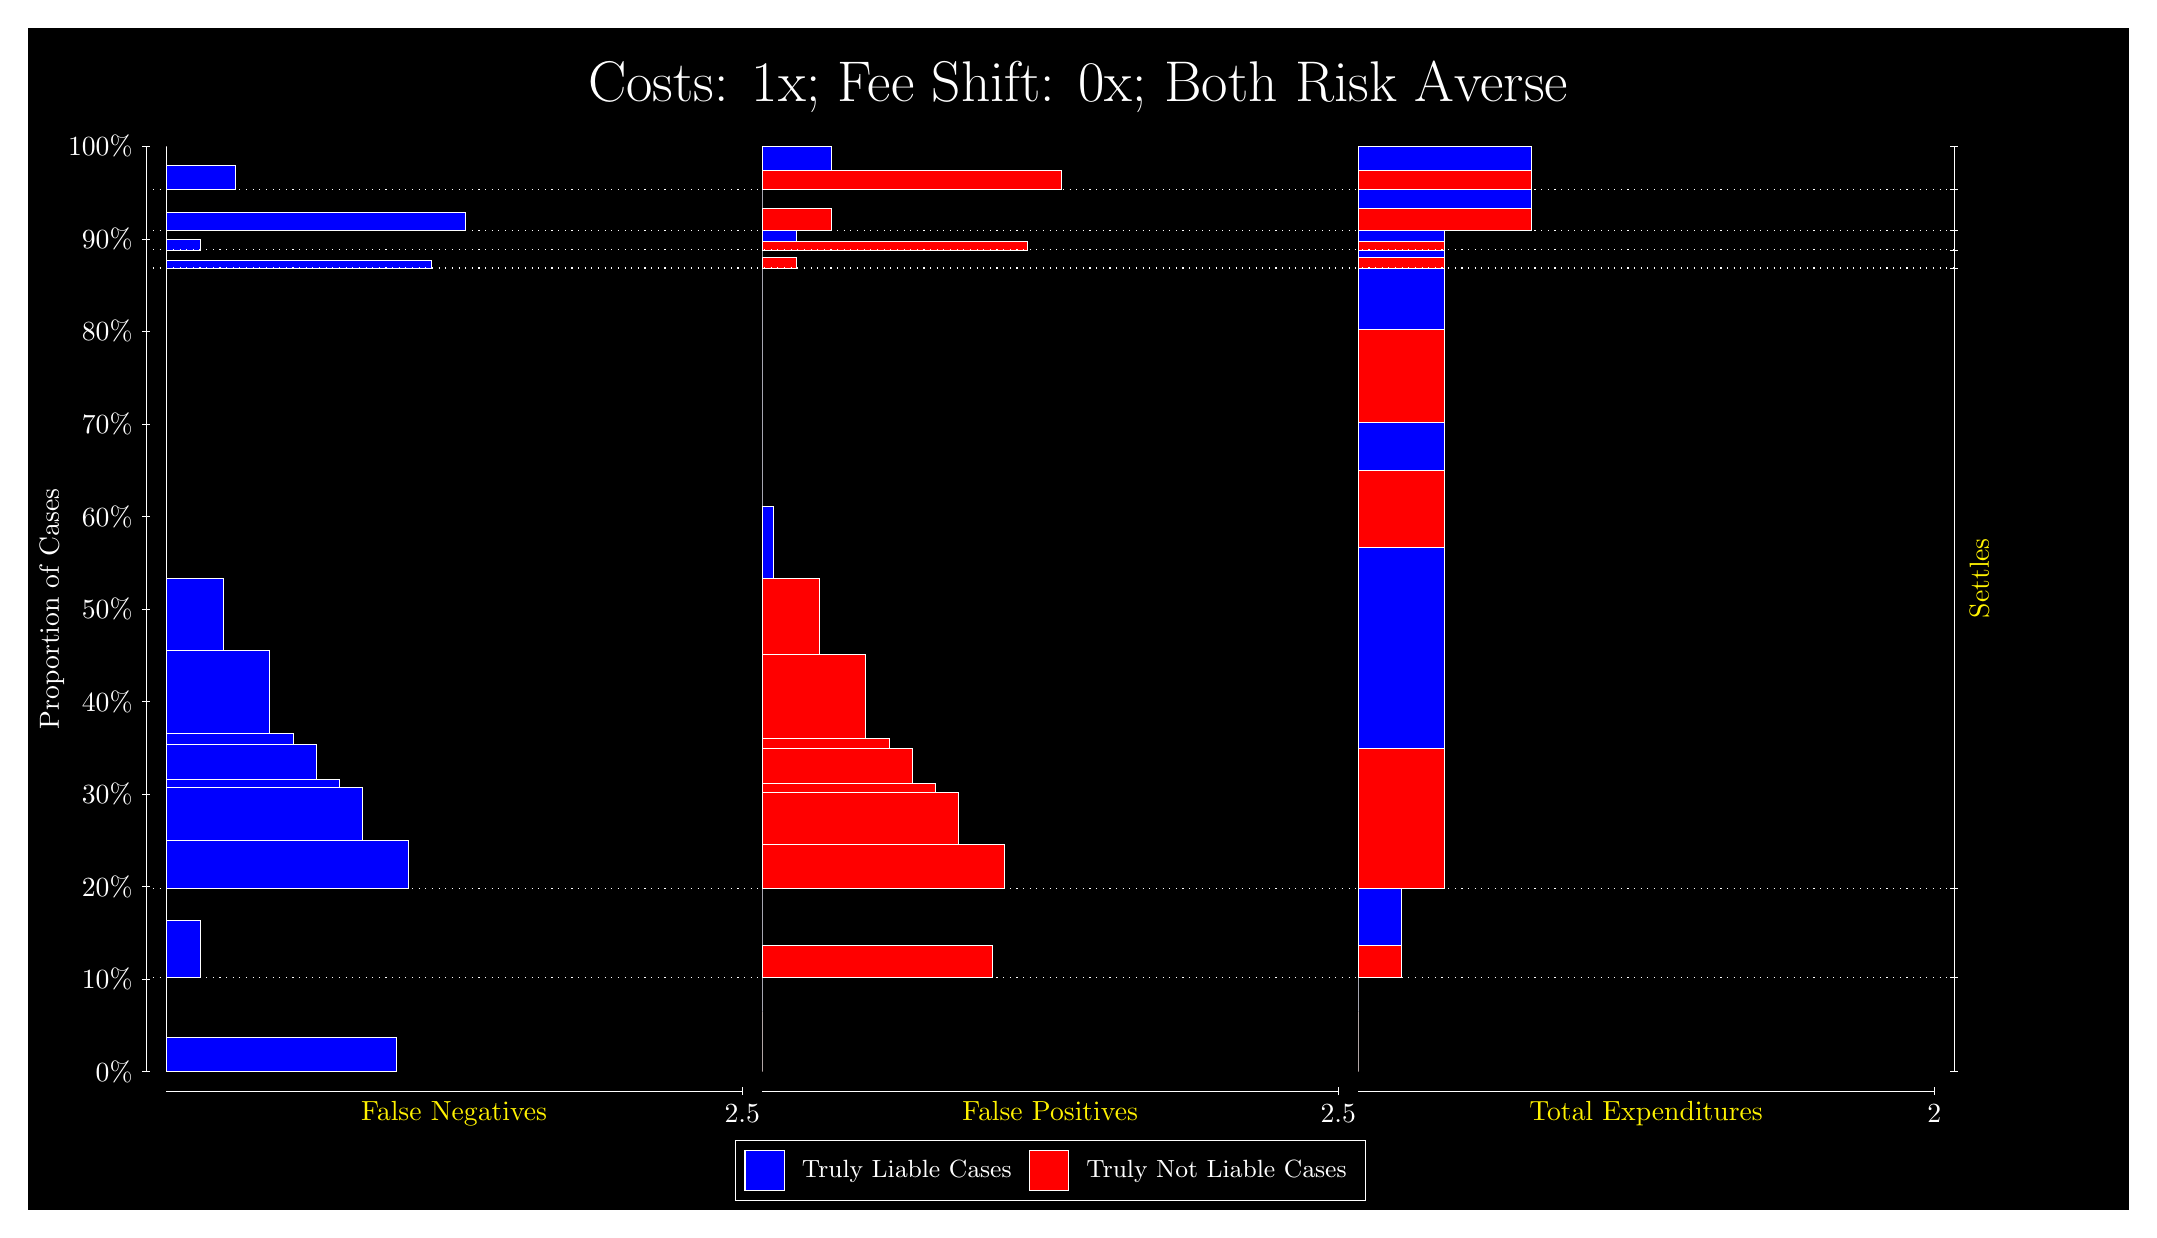
\begin{tikzpicture}
\draw[fill=black] (0,0) rectangle (26.667,15);
\draw[text=white] (0,13.5) rectangle (26.667,15) node[midway] {\huge Costs: 1x; Fee Shift: 0x; Both Risk Averse};
\draw[white, very thin] (1.5,1.75) -- (1.5,13.5);
\node[rotate=90, text=white, anchor=center] at (0.3, 7.625) {Proportion of Cases};
\draw[white, very thin] (1.45,1.75) -- (1.55,1.75);
\node[text=white, anchor=east] at (1.45, 1.75) {0\%};
\draw[white, very thin] (1.45,2.925) -- (1.55,2.925);
\node[text=white, anchor=east] at (1.45, 2.925) {10\%};
\draw[white, very thin] (1.45,4.1) -- (1.55,4.1);
\node[text=white, anchor=east] at (1.45, 4.1) {20\%};
\draw[white, very thin] (1.45,5.275) -- (1.55,5.275);
\node[text=white, anchor=east] at (1.45, 5.275) {30\%};
\draw[white, very thin] (1.45,6.45) -- (1.55,6.45);
\node[text=white, anchor=east] at (1.45, 6.45) {40\%};
\draw[white, very thin] (1.45,7.625) -- (1.55,7.625);
\node[text=white, anchor=east] at (1.45, 7.625) {50\%};
\draw[white, very thin] (1.45,8.8) -- (1.55,8.8);
\node[text=white, anchor=east] at (1.45, 8.8) {60\%};
\draw[white, very thin] (1.45,9.975) -- (1.55,9.975);
\node[text=white, anchor=east] at (1.45, 9.975) {70\%};
\draw[white, very thin] (1.45,11.15) -- (1.55,11.15);
\node[text=white, anchor=east] at (1.45, 11.15) {80\%};
\draw[white, very thin] (1.45,12.325) -- (1.55,12.325);
\node[text=white, anchor=east] at (1.45, 12.325) {90\%};
\draw[white, very thin] (1.45,13.5) -- (1.55,13.5);
\node[text=white, anchor=east] at (1.45, 13.5) {100\%};

\draw[white, very thin] (24.457,1.75) -- (24.457,13.5);
\draw[white, very thin] (24.407,1.75) -- (24.507,1.75);
\node[anchor=west] at (24.407, 1.75) {};
\draw[white, very thin] (24.407,2.9452) -- (24.507,2.9452);
\node[anchor=west] at (24.407, 2.9452) {};
\draw[white, very thin] (24.407,4.0771) -- (24.507,4.0771);
\node[anchor=west] at (24.407, 4.0771) {};
\draw[white, very thin] (24.407,11.955) -- (24.507,11.955);
\node[anchor=west] at (24.407, 11.955) {};
\draw[white, very thin] (24.407,12.186) -- (24.507,12.186);
\node[anchor=west] at (24.407, 12.186) {};
\draw[white, very thin] (24.407,12.428) -- (24.507,12.428);
\node[anchor=west] at (24.407, 12.428) {};
\draw[white, very thin] (24.407,12.952) -- (24.507,12.952);
\node[anchor=west] at (24.407, 12.952) {};
\draw[white, very thin] (24.407,13.5) -- (24.507,13.5);
\node[anchor=west] at (24.407, 13.5) {};

\draw[white, very thin, fill=blue] (1.75,1.75) rectangle (4.6775,2.1838);
\draw[white, very thin, fill=red] (1.75,2.1838) rectangle (1.75,2.9452);
\draw[white, very thin, fill=blue] (1.75,2.9452) rectangle (2.1891,3.6734);
\draw[white, very thin, fill=red] (1.75,3.6734) rectangle (1.75,4.0771);
\draw[white, very thin, fill=blue] (1.75,4.0771) rectangle (4.8239,4.6856);
\draw[white, very thin, fill=blue] (1.75,4.6856) rectangle (4.2384,5.3542);
\draw[white, very thin, fill=blue] (1.75,5.3542) rectangle (3.9457,5.4612);
\draw[white, very thin, fill=blue] (1.75,5.4612) rectangle (3.6529,5.912);
\draw[white, very thin, fill=blue] (1.75,5.912) rectangle (3.3602,6.0427);
\draw[white, very thin, fill=blue] (1.75,6.0427) rectangle (3.0674,7.099);
\draw[white, very thin, fill=blue] (1.75,7.099) rectangle (2.4819,8.0127);
\draw[white, very thin, fill=red] (1.75,8.0127) rectangle (1.75,11.955);
\draw[white, very thin, fill=blue] (1.75,11.955) rectangle (5.1167,12.053);
\draw[white, very thin, fill=red] (1.75,12.053) rectangle (1.75,12.186);
\draw[white, very thin, fill=blue] (1.75,12.186) rectangle (2.1891,12.325);
\draw[white, very thin, fill=red] (1.75,12.325) rectangle (1.75,12.428);
\draw[white, very thin, fill=blue] (1.75,12.428) rectangle (5.5558,12.663);
\draw[white, very thin, fill=red] (1.75,12.663) rectangle (1.75,12.952);
\draw[white, very thin, fill=blue] (1.75,12.952) rectangle (2.6283,13.257);
\draw[white, very thin, fill=red] (1.75,13.257) rectangle (1.75,13.5);
\draw[white, very thin, fill=red] (9.3189,1.75) rectangle (9.3189,2.5114);
\draw[white, very thin, fill=blue] (9.3189,2.5114) rectangle (9.3189,2.9452);
\draw[white, very thin, fill=red] (9.3189,2.9452) rectangle (12.246,3.3489);
\draw[white, very thin, fill=blue] (9.3189,3.3489) rectangle (9.3189,4.0771);
\draw[white, very thin, fill=red] (9.3189,4.0771) rectangle (12.393,4.6326);
\draw[white, very thin, fill=red] (9.3189,4.6326) rectangle (11.807,5.3012);
\draw[white, very thin, fill=red] (9.3189,5.3012) rectangle (11.515,5.4082);
\draw[white, very thin, fill=red] (9.3189,5.4082) rectangle (11.222,5.856);
\draw[white, very thin, fill=red] (9.3189,5.856) rectangle (10.929,5.9867);
\draw[white, very thin, fill=red] (9.3189,5.9867) rectangle (10.636,7.043);
\draw[white, very thin, fill=red] (9.3189,7.043) rectangle (10.051,8.0196);
\draw[white, very thin, fill=blue] (9.3189,8.0196) rectangle (9.4652,8.9333);
\draw[white, very thin, fill=blue] (9.3189,8.9333) rectangle (9.3189,11.955);
\draw[white, very thin, fill=red] (9.3189,11.955) rectangle (9.758,12.088);
\draw[white, very thin, fill=blue] (9.3189,12.088) rectangle (9.3189,12.186);
\draw[white, very thin, fill=red] (9.3189,12.186) rectangle (12.686,12.289);
\draw[white, very thin, fill=blue] (9.3189,12.289) rectangle (9.758,12.428);
\draw[white, very thin, fill=red] (9.3189,12.428) rectangle (10.197,12.717);
\draw[white, very thin, fill=blue] (9.3189,12.717) rectangle (9.3189,12.952);
\draw[white, very thin, fill=red] (9.3189,12.952) rectangle (13.125,13.194);
\draw[white, very thin, fill=blue] (9.3189,13.194) rectangle (10.197,13.5);
\draw[white, very thin, fill=red] (16.888,1.75) rectangle (16.888,2.5114);
\draw[white, very thin, fill=blue] (16.888,2.5114) rectangle (16.888,2.9452);
\draw[white, very thin, fill=red] (16.888,2.9452) rectangle (17.437,3.3489);
\draw[white, very thin, fill=blue] (16.888,3.3489) rectangle (17.437,4.0771);
\draw[white, very thin, fill=red] (16.888,4.0771) rectangle (17.986,5.856);
\draw[white, very thin, fill=blue] (16.888,5.856) rectangle (17.986,8.4075);
\draw[white, very thin, fill=red] (16.888,8.4075) rectangle (17.986,9.3841);
\draw[white, very thin, fill=blue] (16.888,9.3841) rectangle (17.986,9.9925);
\draw[white, very thin, fill=red] (16.888,9.9925) rectangle (17.986,11.18);
\draw[white, very thin, fill=blue] (16.888,11.18) rectangle (17.986,11.955);
\draw[white, very thin, fill=red] (16.888,11.955) rectangle (17.986,12.088);
\draw[white, very thin, fill=blue] (16.888,12.088) rectangle (17.986,12.186);
\draw[white, very thin, fill=red] (16.888,12.186) rectangle (17.986,12.289);
\draw[white, very thin, fill=blue] (16.888,12.289) rectangle (17.986,12.428);
\draw[white, very thin, fill=red] (16.888,12.428) rectangle (19.083,12.717);
\draw[white, very thin, fill=blue] (16.888,12.717) rectangle (19.083,12.952);
\draw[white, very thin, fill=red] (16.888,12.952) rectangle (19.083,13.194);
\draw[white, very thin, fill=blue] (16.888,13.194) rectangle (19.083,13.5);
\draw[white, dotted] (1.5,2.9452) -- (24.457,2.9452);
\draw[white, dotted] (1.5,4.0771) -- (24.457,4.0771);
\draw[white, dotted] (1.5,11.955) -- (24.457,11.955);
\draw[white, dotted] (1.5,12.186) -- (24.457,12.186);
\draw[white, dotted] (1.5,12.428) -- (24.457,12.428);
\draw[white, dotted] (1.5,12.952) -- (24.457,12.952);
\draw[white, very thin] (1.75,1.5) -- (9.0689,1.5);
\node[text=yellow, anchor=north] at (5.4094, 1.5) {False Negatives};
\draw[white, very thin] (9.0689,1.45) -- (9.0689,1.55);
\node[text=white, anchor=north] at (9.0689, 1.45) {2.5};

\draw[white, very thin] (9.3189,1.5) -- (16.638,1.5);
\node[text=yellow, anchor=north] at (12.978, 1.5) {False Positives};
\draw[white, very thin] (16.638,1.45) -- (16.638,1.55);
\node[text=white, anchor=north] at (16.638, 1.45) {2.5};

\draw[white, very thin] (16.888,1.5) -- (24.207,1.5);
\node[text=yellow, anchor=north] at (20.547, 1.5) {Total Expenditures};
\draw[white, very thin] (24.207,1.45) -- (24.207,1.55);
\node[text=white, anchor=north] at (24.207, 1.45) {2};



\node[text=yellow, centered, rotate=90] at (24.777, 8.0161) {Settles};





\draw (12.978300999999998,1.5) node[draw=none] (baseCoordinate) {};
\begin{scope}[align=center]
        \matrix[scale=0.5, draw=white, below=0.5cm of baseCoordinate, nodes={draw}, column sep=0.1cm]{
            \node[rectangle, draw, minimum width=0.5cm, minimum height=0.5cm, fill=blue] {}; &
            \node[draw=none, font=\small, text=white] (B) {Truly Liable Cases}; &
            \node[rectangle, draw, minimum width=0.5cm, minimum height=0.5cm, fill=red] {}; &
            \node[draw=none, font=\small, text=white] (B) {Truly Not Liable Cases}; \\
            };
\end{scope}

\end{tikzpicture}
\end{document}